\section{Framework of Our Approach}\label{sec:framework}
In this section, we propose our out-of-core property graph matching framework.
\subsection{Overview}
Figure~\ref{img:framework} shows the main execution workflow of our framework.
Basically, the framework contains three parts:
\begin{enumerate*}[label={\arabic*.}]
\item Filter on data graph;
\item Compression of intermediate results;
\item Join on compressed data.
\end{enumerate*}
\begin{figure}[ht]
  \centering
  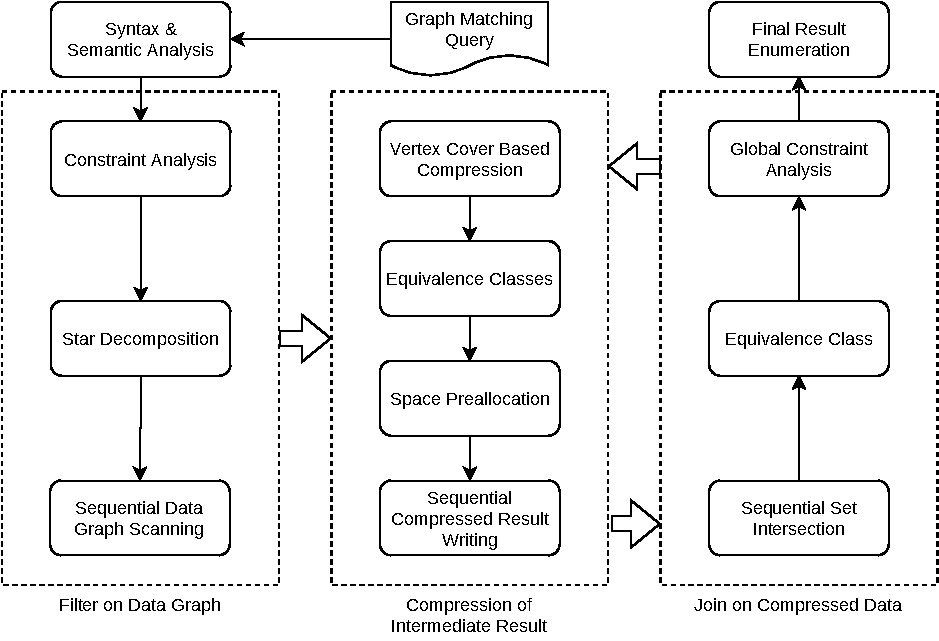
\includegraphics[width=.48\textwidth]{img/framework.pdf}
  \caption{Main Execution Workflow.}\label{img:framework}
\end{figure}
We adopt a join-based method instead of tree-search method to match property graph in an out-of-core environment for two reasons:
Firstly, join-based method is more suitable for real-world graph databases,
the pattern graph is decomposed into smaller parts and matched separately and these partial results can be used as caches for queries afterward;
Secondly, a tree-search method will result in considerable disk I/O because the data vertices are scattered among the disk file.

In order to demonstrate the workflow clearly,
consider the Cypher query in Figure~\ref{img:cypher_query} which corresponds to the pattern graph in Figure~\ref{img:pattern}
(For simplicity, the properties are ignored and use the ID of vertices instead in the WHERE clause).
\begin{figure}[ht]
  \begin{minted}[fontsize=\scriptsize]{cypher}
    MATCH (u1:Person)-[:FOLLOWS]->(u2:Person)-[:FOLLOWS]->(u1),
          (u1)-[:FOLLOWS]->(u3:Person)-[:FOLLOWS]->(u1),
          (u1)-[:PUBLISHES]->(u4:Media), (u1)-[:LIKES]->(u4),
          (u2)-[:LIKES]->(u4)<-[:LIKES]-(u3)
    WHERE id(u1) < id(u2) AND id(u1) < id(u3) AND
          NOT (id(u2) >= id(u3) OR id(u4) >= 2020)
  \end{minted}
  \caption{Graph matching query of the pattern graph in Figure~\ref{img:pattern}.}\label{img:cypher_query}
\end{figure}

\textbf{A graph matching query consists two parts: the pattern graph description part (the MATCH clause) and the constraint specification part (the WHERE clause)}.
It is also possible to support other graph query language if the parser is changed respectively.
The syntax and semantic analyzer would analyze the graph matching query,
check the graph and types, and then generate a valid abstract syntax tree (AST).
Readers interested in these subjects could refer to the textbook~\cite{friedman2001essentials} and we would not discuss it further in this paper.
In the following sections, we will focus on the three main stages of our property graph matching system (as shown in Figure~\ref{img:framework}).

Section~\ref{sec:filter_on_data_graph} describes the first filtering stage, in which we try to reduce not only the output size of the intermediate results,
but also the input size by reading only necessary parts from the huge data graph file.
This is achieved by \textbf{a properly decomposition} of both the constraint specification part (Section~\ref{sec:constraint_analysis})
and the graph description part (Section~\ref{sec:star_decomposition}) of the query,
which is distinct from previous works that our method will hold all structural information that can be used to minimize the disk I/O.
We also design an efficient disk-based \textbf{graph index} (Section~\ref{sec:data_graph_scanning}), such that only one sequential read of the origianl
graph is needed to match all the decomposed atomic query and the preserved structural information
can be used to skip unnecessary parts of the graph.

In Section~\ref{sec:compression_of_intermediate_result}, we demonstrate the data structure that we use to express the intermediate results of graph matching
\textbf{with an extremly high compression ratio}.
Our compression algorithm is based on VCBC~\cite{DBLP:journals/pvldb/QiaoZC17}, and we will give a brief review of the VCBC algorithm in Section~\ref{sec:vcbc}.
To reduce the I/O cost even further, in Section~\ref{sec:equivalence_classes}, we study the \emph{NeighborInfo equivalence classes} in the pattern graphs and use
these equivalence classes to avoid blindly matching result writing. To put theory into practice, one more challenge
is how to write this compressed expression to file without introducing random disk I/O.
To solve this problem, we propose a space pre-allocation method in Section~\ref{sec:space_allocation}.

Finally, Section~\ref{sec:join_on_compressed_data} provides how we join the compressed intermediate results to obtain the
final matching results. To reduce the I/O cost, our algorithm is elegantly designed such that the set intersection
operation could be performed sequentially in linear time (Section~\ref{sec:sequential_set_intersection}).
The space allocation problem still occurred during the join phase, in Section~\ref{sec:space_allocation_eqv} we will address this problem,
and we will show that the equivalence classes can still be applied here to reduce I/O cost further.
At last, in Section~\ref{sec:global_constraint_analysis}, we will describe how to boost the join operation by the user-provided searching conditions.
\subsection{Filter on Data Graph}\label{sec:filter_on_data_graph}
This section describes how we filter on the data graph efficiently by analyzing the user provided searching constraint,
decomposing the pattern graph into stars, and scanning the data graph sequentially.
\subsubsection{Constraint Analysis}\label{sec:constraint_analysis}
The WHERE clause of a graph matching query specified a constraint or searching condition on the matching results.
The constraint are expressed in the form of predicates, e.g., $=$, $\neq$, $>$, $\ge$, $<$, $\le$.
And the Boolean operator AND ($\land$), OR ($\lor$), NOT ($\lnot$) can be used to combine multiple predicates into a new one.
For example, in Figure~\ref{img:cypher_query}, there are three predicates concatenated by AND\@.
Formally, the constraint is a function $\psi: PG \rightarrow B$ with $PG$ the set of pattern graph and $B$ the set of Boolean values.
We will also use $\psi$ to denote abstract predicate for simplicity in this section:
$\psi(u)$ defines a constraint $\psi$ on vertex $u$, e.g., ``\mintinline{cypher}{id(u4) >= 2020}'' defines a vertex constraint on $u_4$ where the ID of the matching vertex of $u_4$ must great than or equal to $2020$;
and $\psi(u_1, u_2)$ defines a constraint on vertex $u_1$ and vertex $u_2$,
e.g., ``\mintinline{cypher}{id(u1) < id(u2)}'' defines a constraint on $u_1$ and $u_2$ that the ID of the matching of $u_1$ must be less than that of $u_2$.

\textbf{Previous work usually ignore the constraint specification part of a graph matching query.}
If someone wants to query a pattern with a specific searching condition,
she or he has to match the pattern graph first and then filter on the matching results,
which leaves a lot of room for improvement because the user provided searching conditions could filter out many unnecessary
partial results in an early phase.

However, it is still challenging to make use of the constraint provided by user's WHERE clause.
The pattern graph and the constraint are logically two different things,
we have to obtain enough information in order to use the constraint as early filter during the graph matching phase.
For example, the constraint in Figure~\ref{img:cypher_query} include all the vertices in the pattern graph,
\textbf{only when the pattern graph is already matched could we got enough information to apply the constraint},
which makes the constraint filter nearly useless.

\begin{figure}[ht]
  \centering
  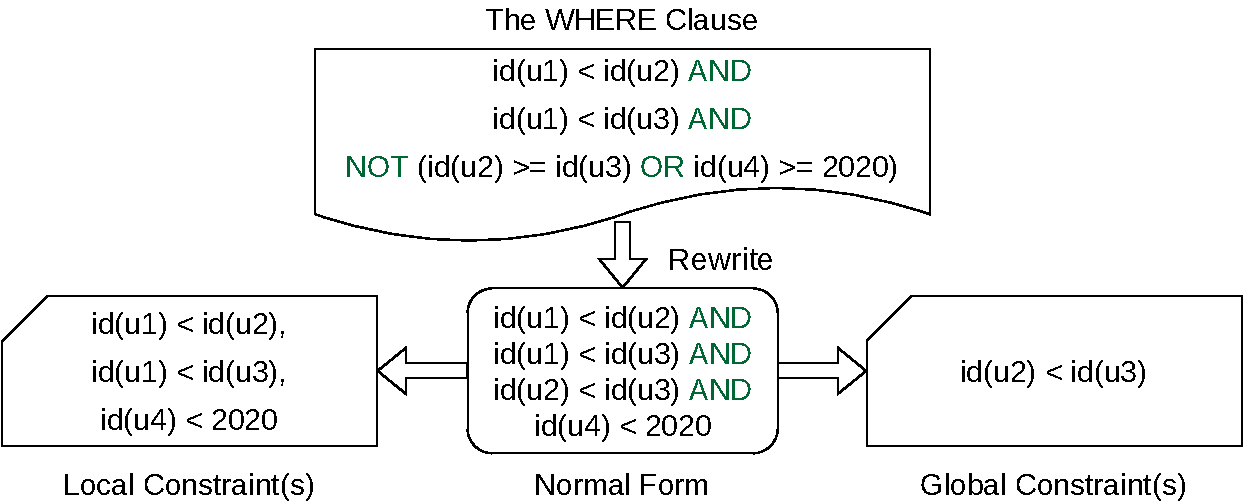
\includegraphics[width=.45\textwidth]{img/constraints.pdf}
  \caption{Constraint Analysis.}\label{img:constraints}
\end{figure}

To address this problem, as shown in Figure~\ref{img:constraints},
we dive into the syntax tree of the graph matching query and decompose the searching condition into smaller parts which require only what we could got during the graph matching phase.
Specifically, we decompose the searching condition into three parts: \emph{vertex constraints}, \emph{edge constraints} and \emph{global constraint}.
A vertex constraint is a function $\psi(u)$ mapping vertex $u$ to Boolean values,
and an edge constraint sets a constraint on edge $(u_1, u_2)$ by a function $\psi(u_1, u_2)$.
For example, in Figure~\ref{img:pattern} ``\mintinline{cypher}{id(u4) < 2020}'' sets a vertex constraint on $u_4$,
``\mintinline{cypher}{id(u1) < id(u2)}'' and ``\mintinline{cypher}{id(u1) < id(u3)}'' are edge constraints,
while ``\mintinline{cypher}{id(u2) < id(u3)}'' is not because there is no edge between $u_2$ and $u_3$.
\textbf{The \emph{vertex constraints} and \emph{edge constraints} are \emph{local constraints} that only require local information that can be obtained during the graph matching phase.
So they could then be pushed down to the data graph scanning phase to short-circuit useless matching results.}
A global constraint $\psi(u_1, u_2, \dots)$ sets a constraint on a series of vertices $u_1, u_2, \dots$,
the information is insufficient during the data graph scanning phase,
however, it still contains many useful information that can be used during the join phase,
and we will discuss it later in Section~\ref{sec:join_on_compressed_data}.

\begin{algorithm}[ht]
  \caption{Constraint Rewriting}\label{alg:rewrite}
  \SetKwFunction{ConstraintRewrite}{\textsc{ConstraintRewrite}}
  \SetKwFunction{Simplify}{\textsc{Simplify}}
  \Input{$expr$: the abstract syntax tree of the WHERE clause}
  \Output{A set of simplified constraints connected by the AND ($\land$) operator}
  \Fn{\ConstraintRewrite{$expr$}}{
    \Match{$expr$}{
      \Case{$\lnot \lnot e$}{\Return{\ConstraintRewrite{$e$}}}
      \Case{$\lnot (e_1 \lor e_2)$}{
        \Return{\ConstraintRewrite{$\lnot e_1$} $\cup$ \ConstraintRewrite{$\lnot e_2$}}
      }
      \Case{$e_1 \land e_2$}{\Return{\ConstraintRewrite{$e_1$} $\cup$ \ConstraintRewrite{$e_2$}}}
      \Case{$e$}{\Return{$\{$ \Simplify{$e$} $\}$}}
    }
  }
\end{algorithm}

Logically, the AND ($\land$) operator create a new constraint $\psi = \psi_1 \land \psi_2$ by combining two constraints $\psi_1$ and $\psi_2$,
where $\psi_1$ and $\psi_2$ can be used to check the matching results independently because there is no side effects in constraints,
so we could safely split $\psi$ into $\psi_1$ and $\psi_2$.
\textbf{Because local constraints are the earliest constraint filters, we should extract as much as possible.}
In order to make the constraint filters more efficient and extract more local constraints:
Firstly, we optimize the AST by classic methods such as compile-time calculation,
handle special cases such as ``\mintinline{cypher}{WHERE false}''.
Then, we apply Algorithm~\ref{alg:rewrite} to analyze the syntax tree and rewrite it into \emph{normal form},
where a normal form is a list of simplified constraints connected by the AND operator.
In fact, the constraints are mostly specified by binary operators such as ``$\le$'', ``$\ne$'',
hence many constraints are naturally local constraints.
And the De Morgan's law enables us to convert the OR ($\lor$) operator into AND ($\land$):
\begin{equation}
  \lnot (\psi_1 \lor \psi_2) = \lnot \psi_1 \land \lnot \psi_2
\end{equation}
So Algorithm~\ref{alg:rewrite} will always keep the semantics of the original user provided constraint.
For example, the third predicate of the AND operator in Figure~\ref{img:cypher_query} would be rewritten to
\begin{minted}[fontsize=\scriptsize]{cypher}
  id(u2) < id(u3) AND id(u4) < 2020
\end{minted}
by applying De Morgan's law.
And the WHERE clause of Figure~\ref{img:cypher_query} would be rewritten to the normal form:
\begin{minted}[fontsize=\scriptsize]{lisp}
  WHERE id(u1) < id(u2) AND id(u1) < id(u3)
  AND id(u2) < id(u3) AND id(u4) < 2020
\end{minted}

\begin{algorithm}[ht]
  \caption{Constraint Pushdown}\label{alg:push_down}
  \SetKwFunction{ConstraintPushdown}{\textsc{ConstraintPushdown}}
  \SetKwFunction{AddVertexConstraint}{\textsc{AddVertexConstraint}}
  \SetKwFunction{AddEdgeConstraint}{\textsc{AddEdgeConstraint}}
  \SetKwFunction{Edges}{\textsc{Edges}}
  \Input{The normal form of constraints $exprs$ and the user described pattern graph $p$}
  \Output{The vertex constraints and edge constraints are pushed down to $p$ and the global constraints will be returned}
  \Fn{\ConstraintPushdown{$exprs$, $p$}}{
    $globals \leftarrow [\,]$\;
    \ForEach{$expr \in exprs$}{
      \Match{$expr$}{
        \Case{$\psi(u)$}{\AddVertexConstraint{$p$, $\psi(u)$}}
        \Case{$\psi(u_1, u_2)$}{
          \If{$(u_1, u_2) \in$ \Edges{$p$}}{\AddEdgeConstraint{$p$, $u_1$, $u_2$, $\psi(u_1, u_2)$}}
        }
        \Case{$e$}{$globals \leftarrow globals \cup \{e\}$\;}
      }
    }
    \Return{$globals$}
  }
\end{algorithm}

The normal form is then used to extract useful information to be pushed down to the pattern graph as in Algorithm~\ref{alg:push_down}.
For each constraint in the normal form, we check if it is local constraint and then push it down to the corresponding vertex or edge.
For example, we would obtain the pattern graph in Figure~\ref{img:pattern_constraint} after doing constraint analysis for the query in Figure~\ref{img:cypher_query}.
After that, We could then decompose it into stars (Section~\ref{sec:star_decomposition}).
Our framework contains a JIT compiler that is able to emit callable closures based on the AST,
and the local constraints can then be used to serve as early filters in the data graph scanning process to short-circuit unnecessary matchings as soon as possible (Section~\ref{sec:data_graph_scanning}).
\begin{figure}[ht]
  \centering
  \resizebox{.7\columnwidth}{!}{
    \begin{tikzpicture}
      \begin{scope}
        \node (C1) at (-3, 1.75) {$C_1: u_1.id < u_2.id$};
        \node (c2) at (3, 1.75) {$C_2: u_1.id < u_3.id$};
        \node (c4) at (3, -2.5) {$C_3: u_4.year < 2020$};
      \end{scope}
      \begin{scope}[every node/.style={circle,thick,draw}]
        \node[label={[label distance=0.6]90:Person}] (1) at (0, 2.25) {$u_1$};
        \node[label={[label distance=1]180:Person}] (2) at (-2.25, 0) {$u_2$};
        \node[label={[label distance=1]0:Person}] (3) at (2.25, 0) {$u_3$};
        \node[label={[label distance=0.6]270:Media}] (4) at (0, -2.25) {$u_4$};
      \end{scope}
      \begin{scope}[>={Stealth[black]},
          every node/.style={fill=white,circle},
          every edge/.style={draw=black}]
        \path [->] (1) edge[bend left=15] node[rectangle,rotate=45] {FOLLOWS} (2);
        \path [->] (2) edge[bend left=15] node[rectangle,rotate=45] {FOLLOWS} (1);
        \path [->] (1) edge[bend left=15] node[rectangle,rotate=-45] {FOLLOWS} (3);
        \path [->] (3) edge[bend left=15] node[rectangle,rotate=-45] {FOLLOWS} (1);
        \path [->] (1) edge[bend left=15] node[rectangle,rotate=-90] {PUBLISHES} (4);
        \path [->] (1) edge[bend right=15] node[rectangle,rotate=-90] {LIKES} (4);
        \path [->] (2) edge node[rotate=-45] {LIKES} (4);
        \path [->] (3) edge node[rotate=45] {LIKES} (4);
      \end{scope}
    \end{tikzpicture}
  }
  \caption{The pattern graph with local constraints pushed down.}\label{img:pattern_constraint}
\end{figure}
\subsubsection{Star Decomposition}\label{sec:star_decomposition}
\textbf{To design a join based graph matching algorithm, the first thing is to decide what is the basic join unit.}
The simplest join unit is edge, however, it will result in huge amount of useless intermediate results if we use edge as basic unit.
Some authors may adopt more complex structure such as frequent subgraphs as their basic unit,
however, super-linear indices are inevitable for these algorithms~\cite{DBLP:journals/pvldb/SunWWSL12},
and this problem would be more severe for out-of-core environment.
Based on these observations, \textbf{we make a balance by adopting star as our basic matching unit},
where a star $S_k$ is a complete bipartite graph $K_{1,k}$ with one root and $k$ leaves.
For one thing, stars can be matched sequentially without complex indices in a out-of-core environment,
which we will discuss more details in the next section.
And for another, stars can hold enough information, both structural information of the pattern graph and the additional searching constraints provided by user's WHERE clause, to reduce the size of intermediate results.
In this section, we will show how to keep these information as much as possible by decompose the pattern graph into stars properly.

\begin{algorithm}[ht]
  \caption{Star Decomposition}\label{alg:decompose_stars}
  \SetKwFunction{DecomposeStars}{\textsc{DecomposeStars}}
  \SetKwFunction{Peek}{\textsc{Peek}}
  \SetKwFunction{Star}{\textsc{Star}}
  \SetKwFunction{RemoveVertex}{\textsc{RemoveVertex}}
  \Input{The pattern graph $p$ with vertex/edge constraints pushed down}
  \Output{A sequence of stars with a specific order}
  \Fn{\DecomposeStars{$p$}}{
    $results \leftarrow [\,]$\;
    $p' \leftarrow p$\;
    $candidates \leftarrow \{u | \max_{u \in \text{Vertices}(p)}f(u)\}$\;
    \While{$candidates \neq \emptyset$}{
      $root \leftarrow$ \Peek{$candidates$}\;
      $candidates \leftarrow candidates \setminus \{ root \}$\;
      $candidates \leftarrow candidates \cup \{ leaf \mid leaf \text{ is adjacent to } root \text{ in } p'\}$\;
      \RemoveVertex{$p'$, $root$}\;
      $candidates \leftarrow candidates \setminus \{ u \mid u \in p' \land \deg{u} = 0 \}$\;
      $results \leftarrow results \cup \{$ \Star{$p$, $root$} $\}$\;
    }
    \Return{$results$}
  }
\end{algorithm}

As many authors have stated before,
\textbf{the matching order has a significant impact on the performance of a graph matching query}~\cite{DBLP:journals/pvldb/SunWWSL12,DBLP:conf/sigmod/HanLL13,DBLP:journals/pvldb/LaiQLC15}.
In our framework, matching order is determined by the stars' root order.
We conclude that the root order affects the overall performance in two aspects:
First, different matching orders result in different join operations which have different performance.
Second, the size of the star matching result is determined by the root selection.
Hence, we provide two rules respectively to guide the star decomposition algorithm (Algorithm~\ref{alg:decompose_stars}):
\begin{itemize}[noitemsep]
\item The root should be selected in the leaves of the previous star except for the first star.
\item We prefer to select the vertex $u$ such that $f(u)$ is the maximum among the candidates,
  where $f(u) = \frac{\deg \times nc}{freq}$ is a heuristic function on the degree $\deg$ of $u$,
  number of constraints $nc$ and the frequency $freq$ of vertices with the same label of $u$ in the data graph.
\end{itemize}

The first rule indicates that the roots would form a connected vertex cover of the original pattern graph step by step.
\textbf{By doing so, the join operation will always occurred between two adjacent stars},
and we could use a simple index to boost the join operation (Section~\ref{sec:join_on_compressed_data}).
In contrast, for example, if the two stars are totally separated without any common vertices,
then the join result of these stars would be the Cartesian product of respective star matching results,
where most of the rows in the Cartesian product would be invalid.
The Second rule considers both the information of the pattern graph and the distribution of data graph.
We prefer to select root that contains more structural constraints ($\deg$) and user provided constraints ($nc$),
and prefer root with a low label frequency in the data graph.
\textbf{By doing so the matching result of the star could be as small as possible which reduces the I/O cost and alleviates the burden of the later join operation.}

Previous work STwig~\cite{DBLP:journals/pvldb/SunWWSL12} and TwinTwig~\cite{DBLP:journals/pvldb/LaiQLC15} also use stars as their basic matching units.
However, unlike these previous work which are designed for simple graphs, our stars fully support the real-world property graph model, and most importantly, we will show that the star decomposition algorithm of previous work has a lot of room to be optimized.

\textbf{Both STwig and TwinTwig are designed for undirected simple graph,
which has a limited expressiveness and is not suitable for many real-world applications.}
In contrast, we adopt the property graph model which is widely used in industrial graph databases.
Figure~\ref{img:stars} shows the decomposition results of the patter graph in Figure~\ref{img:pattern},
both vertices and edges are labeled and multiple edges may exist between a leaf and the root vertex.
The vertex constraint $C_4$ and edge constraints $C_1$, $C_2$ are also shown in the graph.

\begin{figure}[ht]
  \centering
  \resizebox{.6\columnwidth}{!}{
    \begin{tikzpicture}
      \begin{scope}[every node/.style={circle,thick,draw}]
        \node[label={[label distance=0.6]90:Person}] (1) at (0, 2.25) {$u_1$};
        \node[label={[label distance=1]180:Person}] (2) at (-2.25, 0) {$u_2$};
        \node[label={[label distance=1]0:Person}] (3) at (2.25, 0) {$u_3$};
        \node[label={[label distance=0.6]270:Media}] (4) at (0, -2.25) {$u_4$};
      \end{scope}
      \begin{scope}[>={Stealth[black]},
          every node/.style={fill=white,circle},
          every edge/.style={draw=black}]
        \path (1) edge (2);
        \path (1) edge (3);
        \path (1) edge (4);
      \end{scope}
    \end{tikzpicture}
  }
  \resizebox{.6\columnwidth}{!}{
    \begin{tikzpicture}
      \begin{scope}[every node/.style={circle,thick,draw}]
        \node[label={[label distance=1]180:Person}] (2) at (-2.25, 0) {$u_2$};
        \node[label={[label distance=1]0:Person}] (3) at (2.25, 0) {$u_3$};
        \node[label={[label distance=0.6]270:Media}] (4) at (0, -2.25) {$u_4$};
      \end{scope}
      \begin{scope}[>={Stealth[black]},
          every node/.style={fill=white,circle},
          every edge/.style={draw=black}]
        \path (2) edge (4);
        \path (3) edge (4);
      \end{scope}
    \end{tikzpicture}
  }
  \caption{The stars generated by previous algorithms.}\label{img:stars_old}
\end{figure}

\textbf{Apart from the graph model differences, we found that existing query decomposition algorithms still have a a lot of room to be improved.}
As we discussed before, the result of the data graph scanning process should be as small as possible to avoid unnecessary I/O cost.
The leaves of a star graph can be viewed as a bunch of constraints on the root vertex,
which help to eliminate useless mappings of the root.
That is to say: \emph{more leaves, more better}.
However, \textbf{previous work ignore the benefits of leaves and leave a lot of room to be optimized}.
Compared to the decomposition result of previous work in Figure~\ref{img:stars},
our algorithm always keeps all the leaves in the pattern graph,
while, the stars of previous work drop many useful leaves.
In some cases, e.g., triangle graph, they even generate stars with only two vertices which reduce to edge decomposition.
Apparently, an edge will result in much more unnecessary matchings than a star.

The key of the optimization of our algorithm is the use of $p'$:
We first copy the pattern graph $p$ and obtain $p'$.
Then we run the vertex cover finding algorithm on $p'$,
vertices are removed one by one in $p'$ while $p$ is always unchanged.
Finally, we use the original $p$ to induce stars.
So the resulting stars will always hold as much leaves as possible,
which improves the performance of data graph scanning significantly.
Experiments show that this simple optimization can reduce the size of matching results to \@???\% of previous work.
\subsubsection{Data Graph Scanning}\label{sec:data_graph_scanning}
Now, we are ready to elaborate how we match stars efficiently in an out-of-core environment.
First, we will propose our stars matching algorithm by introducing two iterators.
And then we'll show how to implement the two iterators by designing a novel disk format to store the data format,
such that the star matching process is I/O efficient, where \textbf{the huge data graph will be read sequentially without random access, and read at most once}.
\subsubsection*{Stars Matching}
Random disk access problem is always a challenging problem for out-of-core systems,
especially for the out-of-core graph matching problem where graphs are notorious for their poor locality.
However, in this section, we will show that we could avoid random disk accesses by matching stars using two simple iterators.
Furthermore, our techniques ensure that we would only read the necessary part from the huge data graph file,
and these necessary parts would be only read sequentially once.
That is to say, \textbf{we could match all the stars by scanning only the necessary part of the data graph file sequentially once}.

Consider the first star $star_1$ in Figure~\ref{img:stars}, the root vertex is $u_1$ with the label ``Person'',
and it has three leaves $u_2$, $u_3$ and $u_4$.
To match such a star in a data graph, we should find a star whose root also contains the label ``Person''
and it has at least 3 neighbors that could match $u_2$, $u_3$ and $u_4$ respectively.
Then it is straightforward to obtain an naive method to match $star_1$ in a data graph $d$:
Iterate through \textsc{VertexIter}$(d, Person)$ and check every neighbors of these vertices whether they could match $u_2$, $u_3$ and $u_4$, where \textsc{VertexIter}$(d, l)$ travels through all the vertices with the label $l$ in the data graph $d$.
For example, in Figure~\ref{img:data}, $d[v_1]$, the induced graph of $d$ on $v_1$, is such a star that could match $star_1$.

However, this naive star matching method has a great drawback for vertices with a high degree.
Consider the second star $star_2$ in Figure~\ref{img:stars}, the root vertex is $u_4$ with the label ``Media''.
And we suppose that in Figure~\ref{img:data}, $v_4$ is such a popular media that millions or even billions of persons have left their likes.
The naive method have to visit all the neighbors of $v_4$ but most of them are useless because there is no vertex with label ``Comment'' in $star_2$.
To solve this problem, we introduce the second iterator \textsc{NeighborIter}$(v, l)$,
which visits the neighbors with the label $l$ of a given data vertex $v$.
By iterating through \textsc{NeighborIter}$(v_4, Person)$, we could skip useless neighbors and only load the necessary ones.

\begin{definition}[VertexIter and NeighborIter]
  In a data graph $d$, given a vertex label $l$, \textsc{VertexIter}$(d, l)$ is a iterator that would visit all the vertices with the label $l$ in $d$ sequentially.
  Given a data vertex $v$ and a vertex label $l$, \textsc{NeighborIter}$(v, l)$ is a iterator that would iterate through the neighbors with label $l$ of $v$ sequentially.
\end{definition}

Now we will answer the question: How to match the neighbors with the help of \textsc{NeighborIter}?
Consider $star_1$ in Figure~\ref{img:stars}, it is easy to find the symmetry in this star.
We say that $u_2$ and $u_3$ are equivalent because they have the same vertex label,
their connections to the root are the same, and the edge constraints $C_1$ and $C_2$ are also equivalent
(Remember that an edge constraint is a function, that in this case $u_2$ and $u_3$ are just free variables).
For simplicity, we introduce the definition \textsc{NeighborInfo} as follows:
\begin{definition}[NeighborInfo]
  A \textsc{NeighborInfo} of a neighbor vertex $n$ is a structure that stores:
  \begin{enumerate}[noitemsep]
  \item the label of the neighbor $n$,
  \item the vertex constraint of the neighbor $n$,
  \item the edges between the root vertex $v$ and the neighbor $n$
    (the direction of the edges may be $v \rightarrow n$, $v \leftarrow n$ or $v \text{---} n$ because a user could ignore the direction of some edges in the pattern graph),
  \item and the edge constraints of the edges.
  \end{enumerate}
\end{definition}
In a star graph, \textbf{the leaves with the same \textsc{NeighborInfo} form a equivalence class,
and there is no need to blindly permute all possible mappings for the vertices in the same \textsc{NeighborInfo} equivalence class}.
Suppose that there are $m$ leaves with the same \textsc{NeighborInfo} in a star, for each leaf there are $n$ vertices that could be matched in the data graph.
We have to use $m!n$ rows to store the matching result if we blindly permute the mappings for the leaves.
In contrast, only $n$ rows are required if we match group these leaves together which reduces I/O cost dramatically.
\textbf{So instead of matching each neighbors directly, we group the leaves of the star pattern graph by their \textsc{NeighborInfo} during the static analyzing phase, and then use the \textsc{NeighborInfo} to match equivalent vertices at the same time.}
For each neighbor in the \textsc{NeighborIter}, we check whether it would be matched by,
firstly, checking the local constraints of the neighbor,
and then checking the edges between the root and the neighbor.

\begin{algorithm}[ht]
  \caption{Stars Matching}\label{alg:match_stars}
  \SetKwFunction{MatchStars}{\textsc{MatchStars}}
  \SetKwFunction{VertexIter}{\textsc{VertexIter}}
  \SetKwFunction{NeighborIter}{\textsc{NeighborIter}}
  \SetKwFunction{InitializeResults}{\textsc{InitializeResults}}
  \SetKwFunction{AppendResult}{\textsc{AppendResult}}
  \SetKwFunction{FinalizeResults}{\textsc{FinalizeResults}}
  \SetKwFunction{VertexConstraint}{\textsc{VertexConstraint}}
  \SetKwFunction{DegreeConstraint}{\textsc{DegreeConstraint}}
  \SetKwFunction{MatchNeighbor}{\textsc{MatchNeighbor}}
  \SetKwFunction{MatchNeighborInfo}{\textsc{MatchNeighborInfo}}
  \SetKwFunction{Flatten}{\textsc{Flatten}}
  \SetKwFunction{NeighborInfos}{\textsc{NeighborInfos}}
  \Input{The data graph $d$ and a list of $stars$ with the same root label}
  \Output{A list of compressed star matching $results$ corresponding to the $stars$}
  \Fn{\MatchStars{$d$, $stars$}}{
    $results \leftarrow$ \InitializeResults{$stars$}\;
    \ForEach{$v \in$\VertexIter{$d$, $stars[0].root.vlabel$}}{
      $candidates \leftarrow \{ star | star.root$.\VertexConstraint{$v$} $\land star.root$.\DegreeConstraint{$v$} $\}$\;
      $nlabel\_stars \leftarrow $ groups the $candidates$ by leaves' label\;
      \ForEach{$(nlabel, stars) \in nlabel\_stars$}{
        \ForEach{$n \in$\NeighborIter{$v$, $nlabel$}}{
          \MatchNeighbor{$v$, $n$, stars, results}\;
        }
      }
    }
    \FinalizeResults{$results$}\;
    \Return{$results$}\;
  }

  \Fn{\MatchNeighbor{$v$, $n$, $stars$, $results$}}{
    \ForEach{$star \in stars$}{
      \ForEach{$info \in star$.\NeighborInfos{$n.vlabel$}}{
        \If{\MatchNeighborInfo{$v$, $n$, $info$}}{
          \AppendResult{$results[star]$, $n$}\;
        }
      }
    }
  }
\end{algorithm}

By far, there is only one challenge left: How to scan the huge data graph file only once?
The size of the data graph file is proportional to the number of edges in the data graph.
Existing in-memory algorithms would visit the vertices back and forth to explore the data graph,
naively adopt these algorithms to the out-of-core environment would result in numerous swap in/outs,
which is very time consuming and I/O inefficient.
An algorithm that only scan the data graph file sequentially once is desirable,
and we propose a positive answer by providing Algorithm~\ref{alg:match_stars}.
Consider the stars in Figure~\ref{img:stars}, there are two stars that the labels of the roots are different.
\textsc{VertexIter}$(d, Person)$ and \textsc{VertexIter}$(d, Media)$ would be used to visit the vertices in the data graph $d$.
If the data vertices with the same label are stored together in disk,
then the \textsc{VertexIter} could load only the necessary part from disk and visit the vertices sequentially.
Generally speaking, if there are $n$ stars generate by Algorithm~\ref{alg:decompose_stars},
and the size of the labels of the roots is $m$, we have $m \le n$ since multiple stars may have the same label of root.
\textbf{Then we could use $m$ different \textsc{VertexIter} to scan the data graph file by grouping same-label-of-root stars together,
and every iterator would only load a distinct part of the data graph sequentially}
(There is a special case that some stars may isomorphic,
and there is no need to do duplicate star matching, Section~\ref{sec:equivalence_classes} would discuss it in detail).
\textbf{Macroscopically, only the necessary part of the data graph would be loaded to match a pattern graph,
and these parts would be read sequentially only once with the help of \textsc{VertexIter} and \textsc{NeighborIter}.}
\subsubsection*{Data Graph Disk Format}
To implement the two iterators efficiently, we design a compact disk format to store the data graph (Figure~\ref{img:data_disk_format}).
The disk format is a little bit like to the conventional adjacency list format,
that is, we store a vertex and it's neighbors together.

Specifically, in order to implement the \textsc{VertexIter} efficiently,
\textbf{we should locate data vertices efficiently given a vertex label and visit these vertices without random disk access}.
So \textbf{we store vertices with same vertex label adjacently, and adopt a simple label-to-\textsc{VertexIter} index to boost the searching}.
The \mintinline{text}{num_bytes} field would be used to calculate the position of the next data vertex,
such that the \textsc{VertexIter} can visit the data vertices on disk sequentially to reduce I/O cost.
Apart from that, we also store in-degree and out-degree which can be used as early filters during the star matching process.

For the \textsc{NeighborIter}, there is one thing to notice that we adopt the property graph model,
all edges are directed and multi-edges may exist between a pair of vertices.
To store these information, a naive method is to store in-edges and out-edges for each data vertex.
However, this naive method will be very inefficient when matching property graphs.
Consider the pattern graph in Figure~\ref{img:pattern},
suppose that in a data graph $v_1$ matches $u_1$ and we want to check whether $v_2$, a neighbor of $v_1$, matches $u_2$,
then we have to scan all the in-edges to find if there is an edge from $v_2$ to $v_1$ with label ``FOLLOWS'',
and all the out-edges to check if there is an edge from $v_1$ to $v_2$ with the same label.
Real-world graphs usually have a high skewness, for example, a celebrity in a social network may have millions of followers.
\textbf{These ``celebrities'' will become bottleneck if we adopt the naive method to scan all the adjacent edges.}
To solve this problem, we propose a novel schema to store the neighbors,
\textbf{all the edges connected to a neighbor are stored together with the neighbor,
so the neighbor can be checked in place without scanning all the in-edges/out-edges of the root vertex}.
And we also use a simple label-to-\textsc{NeighborIter} index to boost the searching of neighbors given the label of neighbor.
The position of the next neighbor could be calulated by the \mintinline{text}{num_n_to_v} and \mintinline{text}{num_v_to_n} fields.
And we could use \textsc{NeighborIter} to travel through the neighbors sequentially without random disk access.

\begin{figure}[ht]
  \centering
  \begin{minted}[fontsize=\tiny]{text}
+-----------------------------------------+
|             num_vlabels: k              |
+-----------------------------------------+
+-------------+-------------+-------------+
|   vlabel    |     pos     |     len     |<-+
+-------------+-------------+-------------+  |
|   vlabel    |     pos     |     len     |  |
+-------------+-------------+-------------+  |- k rows
                    ...                      |
+-------------+-------------+-------------+  |
|   vlabel    |     pos     |     len     |<-+
+-------------+-------------+-------------+
+--------------------+--------------------+
|     num_bytes      |         v          |<-----------------------------+
+--------------------+--------------------+                              |
|      in_deg        |      out_deg       |                              |
+--------------------+--------------------+                              |
|               num_vlabels               |                              |
+-----------------------------------------+                              |
+-------------+-------------+-------------+                              |
|   vlabel    |     pos     |     len     |<-+                           |
+-------------+-------------+-------------+  |                           |
|   vlabel    |     pos     |     len     |  |                           |
+-------------+-------------+-------------+  |- num_vlabels rows         |
                    ...                      |                           |
+-------------+-------------+-------------+  |                           |
|   vlabel    |     pos     |     len     |<-+                           |
+-------------+-------------+-------------+                              |     One
+-----------------------------------------+                              |- VertexNode
|                    n                    |                              |
+--------------------+--------------------+                              |
|    num_n_to_v      |    num_v_to n      |                              |
+--------------------+--------------------+                              |
+-----------------------------------------+                              |
|                 elabel                  |<-+                           |
+-----------------------------------------+  |                           |
|                 elabel                  |  |  num_n_to_v + num_v_to_n  |
+-----------------------------------------+  |-           rows           |
                    ...                      |                           |
+-----------------------------------------+  |                           |
|                 elabel                  |<-+                           |
+-----------------------------------------+                              |
                    ...                    <-----------------------------+

  \end{minted}
  \caption{Data graph disk format. (TODO\@: Update this figure.)}\label{img:data_disk_format}
\end{figure}

The vertices are sorted by their ID in the data graph, which is very helpful for the join operation (Section~\ref{sec:join_on_compressed_data}).
Given a series of vertices and a series of edges with arbitrary order,
the data graph file could be generated in sorting time.
And for simplicity, we ignore the key-value properties of a property graph and focus on the labels.
In fact, these properties can be added to our disk format by simply add the corresponding fields.
And the simplicity of the \textsc{VertexIter} and \textsc{NeighborIter} also makes it possible to implement them on other platform, e.g., industry-tested relational database, which we will study in future work to make dynamic property graph transactions and analysis easier.
\subsection{Compression of Intermediate Result}\label{sec:compression_of_intermediate_result}
In this section, we describe our efforts to reduce the I/O cost of materializing intermediate results by compression.
Since both the star matching results and the join results are compressed,
to make it clearly, we'll focus on the compression of star matching results in this section,
and leave the compression of join results in Section~\ref{sec:join_on_compressed_data}.
Firstly, we'll give a brief review of the theoretical VCBC algorithm in Section~\ref{sec:vcbc},
and then provide our contributions to make it practical for out-of-core environment in the following subsections.
\subsubsection{Vertex Cover Based Compression}\label{sec:vcbc}
Recall that in Definition~\ref{def:property_graph_matching},
the property graph matching problem is to report the set $\mathcal{I}$.
If we specify an order on the vertices of the pattern graph $P$,
then $\mathcal{I}$ could be represented by a sequence of rows with each row containing the vertices in $D$ that match the vertices in $P$ with the order we specified.
The space to store $\mathcal{I}$ is proportional to the number of matching graphs if we store these rows naively.
Unfortunately, the size of matching result is super-linear with respect to the size of the data graph.
Thus, a compression algorithm with a significant compression ratio is required to reduce the I/O cost for materializing the intermediate matching results.
The \emph{vertex cover based compression} (VCBC)~\cite{DBLP:journals/pvldb/QiaoZC17} algorithm is such an attempt to resolve the output crisis of graph matching using output compression.

The authors of VCBC define the \emph{helve} of an instance of $P$,
where the instance $F$ is a subgraph of the data graph $D$ such that $F \cong P$.
\begin{definition}[Helve]
  Let $V_C = \{u_1, u_2, \dots, u_k\}$ be a vertex cover of $P$.
  Let $F$ be an instance of $P$.
  The helve of $F$ is the vertored images of $V_C$ under the instance-bijection $f_F$:
  \[\mathcal{H}_{V_C}(F) = (f_F(u_1), f_F(u_2), \dots, f_F(u_k))\]
  It is also denoted as $\mathcal{H}(F)$ if $V_C$ is obvious in the context.
  Similarly, the helves of an instance set $\mathcal{I}$ is defined as
  \[\mathcal{H}(\mathcal{I}) = \{\mathcal{H}(F) | F\in \mathcal{I}\}\]
\end{definition}
Let $h_1, h_2, \dots, h_l$ be the $l$ helves in $\mathcal{H}(\mathcal{I})$,
the compression of $\mathcal{I}$ could then be obtained in the following steps:
\begin{enumerate}[noitemsep]
\item Define the \emph{conditional instance set} $\mathcal{I}|h_i$ of $h_i$ as
  \[ \mathcal{I}|h_i = \{F | \mathcal{H}(F) = h_i\} \]
\item For $\mathcal{I}|h_i$,
  identify the \emph{conditional image set} $\operatorname{Img}_P(u|h_i)$ for each vertex $u \in V(P)$:
  \[ \operatorname{Img}_P(u|h_i) =\{f_F(u) | F \in (\mathcal{I}|h_i)\} \]
\item Compress $\mathcal{I}|h_i$ with the concatenation of the conditional images $\operatorname{Img}_P(u|h_1)$ for all vertices in $V(P)$, and we name $\operatorname{code}(\mathcal{I}|h_i)$ as \textsc{SuperRow} in this paper:
  \[ \operatorname{code}(\mathcal{I}|h_i) = \{ \operatorname{Img}(u|h_i) | u \in V(P) \} \]
\item Obtain the VCBC $\operatorname{code}(\mathcal{I})$ by concatenation:
  \[ \operatorname{code}(\mathcal{I}) = \{ \operatorname{code}(\mathcal{I}|h_i) | i \in [1,l]\} \]
\end{enumerate}
For a star graph, the root is the vertex cover.
For example, in Figure~\ref{img:stars}, $u_1$ and $u_4$ are the roots and the vertex cover.

The decompression process works as follows to restore $\mathcal{I}$ from $\operatorname{code}(\mathcal{I})$:
\begin{enumerate}[noitemsep]
\item For each $\operatorname{code}(\mathcal{I}|h_i)$, let $S$ be the Cartesian product over the image sets:
  \[ S = \prod_{u \in V(P)} \operatorname{Img}(u | h_i) \]
\item Let $\mathcal{I}'|h_i$ be the set of tuples in $S$ without duplicated vertices that are validated by the searching condition $\psi$
\item Finally, $\mathcal{I}' = \bigcup_{i \in [1, l]}(\mathcal{I}'|h_i)$ is the decompressed matching result.
\end{enumerate}

VCBC is lossless such that $\mathcal{I}' = \mathcal{I}$~\cite{DBLP:journals/pvldb/QiaoZC17}.
The data compression ratio of VCBC $\rho(\mathcal{I})$ could be calculated by
\[ \rho(\mathcal{I}) = \frac{|\mathcal{I}|}{|\operatorname{code}(\mathcal{I})|} \]
In fact, the compression ratio could have several orders of magnitude since VCBC postpone the resource consuming Cartesian product to the decompression stage.

There is one thing to note that, the VCBC algorithm only introduce a theoretical method to compress the matching results.
\textbf{For a real-world out-of-core environment, many practical challenges have to be solved},
for example, how to design the disk format to store the VCBC compressed data efficiently?
How to write the compressed data sequentially to disk?
And how to decompress the VCBC data file in a sequential manner?
These challenges would be solved in the following two subsections.
\subsubsection{NeighborInfo Equivalence Classes}\label{sec:equivalence_classes}
VCBC save the space by postponing the Cartesian product,
however, this is not the only way to save space.
In this subsection, we discuss how to reduce the size of matching results further by finding equivalence classes in the pattern graph, and finally introduce the disk format of our compressed data.

In Section~\ref{sec:data_graph_scanning}, we introduce the concept \textsc{NeighborInfo}.
In a star graph $S$, suppose that the leaves $n_1, n_2, \dots, n_k$ have the same \textsc{NeighborInfo},
then their conditional image set would also be the same $\operatorname{Img}_S(n_1 | h_i) = \operatorname{Img}_S(n_2 | h_i) = \cdots = \operatorname{Img}_S(n_k | h_i)$ because of symmetry.
These leaves are equivalent under the relation ``has the same \textsc{NeighborInfo}'',
so we could store the image set only once.
This technique is of great importance for ``celebrity'' rooted stars,
otherwise we have to store the numerous followers multiple times.

For some pattern graph, e.g., complete undirected graph with all the vertices and edges share the same label,
the stars decomposed from it would always be the same.
Formally, we say that these stars are equivalent under the relation ``has the same \textsc{Characteristic}'',
where the \textsc{Characteristic} is defined as follows:
\begin{definition}[Characteristic]
  A \textsc{Characteristic} of a star $S$ is a tuple $(\psi, l, N)$, where:
  \begin{enumerate}[noitemsep,label={(\arabic*)}]
  \item $\psi$ is the vertex constraint for the root of $S$.
  \item $l$ is the label of the root of $S$.
  \item $N = \{ \textsc{NeighborInfo}(n) | n \in S.leaves\}$ is a set of \textsc{NeighborInfo}s of the leaves in $S$.
  \end{enumerate}
\end{definition}
Apparently, isomorphic stars have the same \textsc{Characteristic}.
These equivalent stars could be matched once for all,
and the matching results could be stored only once.

\textbf{The previous \textsc{NeighborInfo} and \textsc{Characteristic}
are two basic equivalence classes that can be used to avoid duplication in the star matching results.}
In Section~\ref{sec:join_on_compressed_data} we will show that these equivalence classes can also be used to reduce I/O cost for joined results.
Before that, we will discuss how to design the disk format for the compressed data.
Figure~\ref{img:result_disk_format} shows the disk format of our compressed matching result.
Theoretically, the VCBC compressed data is a sequence of \textsc{SuperRow}s,
where each \textsc{SuperRow} contains a list of conditional image sets $\operatorname{Img}_P(u | h_i)$ for $u \in V(P)$.
However, \textbf{because of the \textsc{NeighborInfo} equivalence class, we don't have to store all the conditional image sets}.
To address this problem, we group the vertices by their \textsc{NeighborInfo} and store the conditional image set for each \textsc{NeighborInfo} instead.
For each conditional image set, we store the starting position \mintinline{text}{pos} and the size of the set \mintinline{text}{len}, and the elements are stored at the end of each \textsc{SuperRow}.
\begin{figure}[ht]
  \centering
  \begin{minted}[fontsize=\tiny]{text}
+-------------+-------------+-------------+
|   num_rows  |   num_eqvs  |  num_cover  |
+-------------+-------------+-------------+
+-----------------------------------------+
|                num_bytes                |<------------------+
+-----------------------------------------+                   |
+--------------------+--------------------+                   |
|         pos        |         len        |<-+                |
+--------------------+--------------------+  |                |
|         pos        |         len        |  |                |
+--------------------+--------------------+  |- num_eqvs rows |
                    ...                      |                |
+--------------------+--------------------+  |                |
|         pos        |         len        |<-+                |- One SuperRow
+--------------------+--------------------+                   |
+-----------------------------------------+                   |
|                    v                    |                   |
+-----------------------------------------+                   |
|                    v                    |                   |
+-----------------------------------------+                   |
                    ...                                       |
+-----------------------------------------+                   |
|                    v                    |<------------------+
+-----------------------------------------+
  \end{minted}
  \caption{Disk format for compressed matching result.}\label{img:result_disk_format}
\end{figure}
\subsubsection{Space Allocation}\label{sec:space_allocation}
In Section~\ref{sec:data_graph_scanning} we showed that during the star matching process,
the data graph file would only be read sequentially at most once without random disk access.
Now in this subsection, \textbf{we will show that the matching result of stars would also be written sequentially with new data appended to the result file}.

For a star graph $S$, the vertex cover is the root, so the first image set for each \textsc{SuperRow} always contains only one element and this is the helve $h_i$.
However, for the leaves in the star, the length of their image sets could only be known after all the neighbors of the helve are scanned in the data graph.
That is to say, $|\operatorname{Img}_S(n|h_i)|$ would be known only if $\operatorname{Img}_S(n|h_i)$ is already written to file for $n \in S.leaves$.

To address this dilemma, a naive approach may allocate buffers in core to store the temporary data and then write these buffers to file.
\textbf{However, this naive approach is very inefficient for the copy, and most of all,
these temporary data could even be larger than the size of the main memory
because real-world graph are skewed and ``celebrities'' may have millions or even billions of followers.}
Thus, it is desirable to write the image sets direct to disk file.
For this purpose, \textbf{we propose a space allocation algorithm to allocate space for image sets ahead of time}.
Specifically, for each vertex in data graph, we store its neighbors together with the vertex and the neighbors are grouped by the vertex label (Section~\ref{sec:data_graph_scanning}).
For each group, the number of vertices are stored in the data graph file and this number is the upper bound of the corresponding image set, because these vertices are filtered and then write to the image set.
Based on this observation, we could allocate enough space to store the image sets ahead of time.
And with the help of \textsc{NeighborIter}, the neighbors are checked sequentially and then write to the proper place in the result file.
\textbf{The operating system would keep at most \mintinline{text}{num_eqvs} pages to write the image sets,
and the elements could be written sequentially to each of these pages.}
\subsection{Join on Compressed Data}\label{sec:join_on_compressed_data}
Theoretically~\cite{DBLP:journals/pvldb/QiaoZC17}, the join operation is performed as in Algorithm~\ref{alg:join_theory}.
However, \textbf{there are many challenges have to be conquered to implement it in an out-of-core environment efficiently},
i.e., How to implement the set intersection operation such that the I/O cost could be minimized?
How to write the result of the join operation in an sequential manner without frequent random disk access?
And how to apply the user-provided searching conditions to boost the join operation?
In this section, we'll answer these problems in detail.
\begin{algorithm}[ht]
  \caption{Join algorithm in theory.}\label{alg:join_theory}
  \SetKwFunction{JoinFun}{\textsc{Join}}
  \Input{A helve $h$ for an instance of the pattern graph $p$, a sequence of stars $\mathcal{P} = \{p_1, p_2, \dots, p_\lambda\}$ decomposed from $p$,
    for each star $p_i \in \mathcal{P}$, projections $h_i$ on $p_i$ and conditional code $\operatorname{code}(\mathcal{I}_{p_i} | h_i)$.}
  \Output{$\operatorname{code}(\mathcal{I}_p|h)$.}
  \Fn{\JoinFun{$h$, $p$, $\mathcal{P}$, $\{\operatorname{code}(\mathcal{I}_{p_i}|h_i) | i \in [1, \lambda]\}$}}{
    \ForEach{$u \in V(p)$}{
      $\operatorname{Img}_p'(u|h) \leftarrow \bigcap_{i \in [1, \lambda] \land u \in V(p_i)}\operatorname{Img}_{p_i}(u|h_i)$\;
    }
    $\operatorname{code}(\mathcal{I}_p | h) \leftarrow $ apply the compression algorithm in Section~\ref{sec:vcbc}\;
    \Return{$\operatorname{code}(\mathcal{I}_p | h)$}\;
  }
\end{algorithm}
\subsubsection{Sequential Set Intersection}\label{sec:sequential_set_intersection}
The authors of VCBC do not draw much attention on the set intersection operation in Algorithm~\ref{alg:join_theory}
because they assume that these operations are performed in memory~\cite{DBLP:journals/pvldb/QiaoZC17}.
Given two image sets $s_1$, $s_2$ with $|s_1| \ge |s_2|$,
a straightforward approach to compute $s_1 \cap s_2$ is to load these sets into memory and convert $s_1$ into hash table,
then iterate through $s_2$ and check existence in the hash table $s_1$.
\textbf{However, as illustrate in Algorithm~\ref{alg:join_theory}, the set intersection operation is the innermost operations in the loop, and it could become the bottleneck if not handled properly.}
Consider the social media network,
the trending media could easily attract millions or even billions of viewers,
to join on such trending media rooted stars,
billions of viewers have to be loaded into memory and converted into hash table to perform the set intersection,
which could easily eat up the memory for a PC and have poor locality because of the hash table.
\textbf{A sequential approach with linear time performance is desirable.}

To address this challenge, we provide an out-of-core sequential approach.
Suppose that if both $s_1$ and $s_2$ are sorted, then $s_1 \cap s_2$ could be obtained by a merge operation,
the elements in $s_1$ and $s_2$ could be scanned sequentially in disk and there is no need to load them entirely into memory and there is no overhead to create the hash table.
However, $s_1$ and $s_2$ must be sorted ahead of time otherwise the time consuming sorting operation could lead to disaster.
Now let's check the data graph scanning phase in Section~\ref{sec:data_graph_scanning}.
The elements in $\operatorname{Img}_{p_i}(u | h_i)$ are in fact written by filtering the \textsc{NeighborIter} sequentially.
If the \textsc{NeighborIter} visits the vertices in a sorted order, then every $\operatorname{Img}_{p_i}(u | h_i)$ is also sorted consequently.
In fact, this is a byproduct since our data graph file is elegantly designed such that the vertices are sorted by their Id, so the order always preserves.
\textbf{Thus we could implement our sequential out-of-core set intersection for free.}
\subsubsection{Space Allocation \& NeighborInfo Equivalence Classes}\label{sec:space_allocation_eqv}
As in Section~\ref{sec:space_allocation}, the space allocation problem still occurs during the join phase since the join result is also compressed.
For $u \in V(p)$, we would write $\operatorname{code}_p(u | h) = \operatorname{code}_{p_1}(u | h_1) \cap \operatorname{code}_{p_2}(u | h_2)$ to the intermediate result file as illustrate in Algorithm~\ref{alg:join_theory}.
However, the size of $\operatorname{code}_p(u | h)$ is not known until the set intersection operation is done.
To address this problem and make the out-of-core sequential intersection discussed in the previous subsection doable,
we estimate the upper bound for $|\operatorname{code}_p(u | h)|$ similar to the approach in Section~\ref{sec:space_allocation}.
This time, the upper bound is estimated as
\[ \min{|\operatorname{code}_{p_1}(u | h_1)|, |\operatorname{code}_{p_2}(u | h_2)|}\]
since the cardinality of interaction could not be greater than the cardinality of the smallest set.
Thus, the space to store the image sets could be allocated before the set intersection operation,
and \textbf{the join result could then be written to these specific positions sequentially without random disk access or redundant memory buffer}.

During the star matching phase, the \textsc{NeighborInfo} equivalence class makes it possible to combine multiple leaves together and store the image set only once, which saves more space and reduces the I/O cost further.
Now we will show that \textbf{NeighborInfo equivalence classes also exist in the join phase}.
Consider the two stars $p_1$ and $p_2$ in Figure~\ref{img:stars},
$u_2$ and $u_3$ belong to the same \textsc{NeighborInfo} equivalence class in both of the stars respectively,
i.e., for a helve $h$ and its projections $h_1$, $h_2$,
we have
\begin{align*}
  \operatorname{Img}_{p_1}(u_2 | h_1) &= \operatorname{Img}_{p_1}(u_3 | h_1) \\
  \operatorname{Img}_{p_2}(u_2 | h_2) &= \operatorname{Img}_{p_2}(u_3 | h_2)
\end{align*}
Consequently,
\[\operatorname{Img}_{p_1}(u_2 | h_1) \cap \operatorname{Img}_{p_2}(u_2 | h_2) = \operatorname{Img}_{p_1}(u_3 | h_1) \cap \operatorname{Img}_{p_2}(u_3 | h_2)\]
which means the equivalence class also hold in the join phase.
Formally, if $u_1, u_2, \dots, u_k \in V(p_i)$ belong to the same equivalence class $\mathcal{C}_i$ in $p_i$,
and $u_1, u_2, \dots, u_k \in V(p_j)$ belong to the same equivalence class $\mathcal{C}_j$ in $p_j$,
then we have
\[ \operatorname{Img}_{p_i \cup p_j}(\mathcal{C} | h) = \operatorname{Img}_{p_i}(\mathcal{C}_i | h_i) \cap \operatorname{Img}_{p_j}(\mathcal{C}_j | h_j) \]
where $p = p_i \cup p_j$ is the composition of $p_i$ and $p_j$, i.e.,
$V(p) = V(p_i) \cup V(p_j)$, $E(p) = E(p_i) \cup E(p_j)$.
And we could use $\operatorname{Img}_{p_i \cup p_j}(\mathcal{C} | h)$ to represent the image set of $u_1, u_2, \dots, u_k$,
\textbf{which reduces the I/O cost to write the join results}.
\subsubsection{Global Constraint Analysis}\label{sec:global_constraint_analysis}
Constraints can be applied only if enough information could be obtain,
so we left the global constraints in Section~\ref{sec:filter_on_data_graph}.
Now in the subsection, we are ready to study the global constraints.

Consider the Cypher query in Figure~\ref{img:cypher_query}, if the WHERE clause is replaced by:
\begin{minted}{cypher}
WHERE id(u1) < id(u2) OR id(u4) < id(u2)
\end{minted}
Then in this case, we could not simplify it anymore because the two predicates are connected by the ``OR'' operator not the ``AND'', and the De Morgan's law is not helpful.
This is a global constraint and it cannot be used to filter the vertices during the star matching process.
Suppose that we want to match the first star $p_1$ in Figure~\ref{img:stars},
and $v_{10}$ in the data graph is the helve, i.e., $v_{10}$ matches the root $u_1$,
and we want to check whether the neighbor of $v_{10}$, say $v_{5}$, could match $u_2$ or $u_3$.
Then the first predicate \mintinline{cypher}{id(u1) < id(u2)} would certainly fail ($10 > 5$) but we cannot simply say that $v_5$ cannot match $u_2$ because the second predicate \mintinline{cypher}{id(u4) < id(u2)} may be true.
The point here is that we do not have enough information about $u_4$ and we could not use this global constraint to boost the star matching process.

\textbf{This dilemma could be resolved in the join phase if only we have got enough information.}
Consider also the case in Figure~\ref{img:stars}, we got the original pattern graph from the two stars after the join process, and $u_1$, $u_4$ is the vertex cover.
That is to say, a helve $h$ is a vector of two vertices in the data graph that matches $u_1$ and $u_4$ respectively,
for example, $h = (v_{10}, v_4)$.
Now, the global constraint \mintinline{cypher}{id(u1) < id(u2) OR id(u4) < id(u2)} is able to filter the image set of $u_2$ since we have already known that $u_1 \mapsto v_{10}$ and $u_4 \mapsto v_4$, only $u_2$ is the free variable.
Formally, a global constraint $\psi(u_1, u_2, \dots, u_k, u_{k+1})$ is a user defined function on a set of vertices $\{u_1, u_2, \dots, u_k, u_{k+1}\}$.
If $u_1, u_2, \dots, u_k$ are the roots of the stars, then these vertices are the vertex cover for the new joined graph and the image sets of these vertices form the helve, and $u_{k+1}$ is the only free variable in $\psi$.
\textbf{So we could use $\psi$ to filter on the image set of $u_{k+1}$,
which helps reduce the size of the join result and avoid useless mappings in an early phase.}

However, there are some global constraints that cannot be applied during the join phase,
for example, the \mintinline{cypher}{id(u2) < id(u3)} we left in Section~\ref{sec:constraint_analysis}.
As we discussed just before, the constraint have to relate to a vertex cover such that it could be used boost the star matching or join process.
This constraint is unique because there are no edges between $u_2$ and $u_3$.
\textbf{From a practical point of view,
it makes sense to provide extra constraints on connected vertices because these connections have concrete meanings,
and if a user provide a self defined relationship irrelevant to the topology of the pattern graph, she or he is highly likely to expect it works as deduplicator to remove duplicate results because of the symmetry in the pattern graph},
and this is the case in our example.
In fact, as is shown in Figure~\ref{img:pattern_constraint}, there is no difference between $u_2$ and $u_3$ in the pattern graph.
In the previous subsection we have shown that $u_2$ and $u_3$ share a common image set in the join result,
so in fact there is no need to apply the \mintinline{cypher}{id(u2) < id(u3)} constraint in the join phase.
This kind of constraint could just be used during the decomposition process to obtain the final results.
